%!TEX TS-program = pdflatex
%!TEX encoding = UTF-8 Unicode
%!TEX TS-options = -halt-on-error
\chapter{Implementation} % (fold)
\label{cha:implementation}

The \gls{EDISON} system that was already used in \autoref{ch:algorithm_analysis}
for analysis was the base for the implementation respectively the porting
process. \Gls{EDISON} is build around the mean shift method and offers
functionality to filter, segment images and edge detection. The complete
software is rather complex having a scripting engine, \gls{GUI} and different
versions of the filtering step, where each step is introducing some technique
to accelerate the filtering. Furthermore the filtering was construed to analyze
feature spaces with arbitrarily dimensions, different kernels, weight maps and 
so on. 

Since the focus of this work is on image segmentation only the filtering
functions and some segmentation helper functions were taken from \gls{EDISON} as
reference. The image loading, saving, pre-, postprocessing and the filtering
part, which is the most compute intensive part with 99.1\% (from
\autoref{tab:comped}) of the run-time, were completely rewritten whereas the
clustering, labeling and elimination of spatial regions (see \autoref{alg:mss})
with in sum 0.9\% of the run-time were adopted without change.

As mentioned before there are three algorithms of the filtering step. For the
purpose of this work the standard mean shift algorithm was choosen because (1)
it is the most compute intensive and (2) it has the best quality output. The other
two versions of the algorithm induce a quality loss and use structures to 
accelerate the algorithm that are not well suited for the \gls{GPU}. Additionally
the compute power of a \gls{GPU} is more visible with the first version. 

\section{Reference Implementation} % (fold)
\label{sec:reference_implementation}

The first step was to do a reference implementation on the \gls{CPU}. The
\gls{CPU} programming framework has better debugging and logging facilites
than a \gls{GPU}. It is not possible to do a system call like \textsf{printf}, 
\textsf{fopen} on a \gls{GPU} which makes debugging hard and logging rather 
impossible. 

The idea behind the reference implementation was to have a running code which is
doing the segmentation in the \emph{right} way. The advantage of this is that
when porting to the \gls{GPU} there is always a reference to which the results
of a \gls{GPU} run can be compared too. This way it is assured that the
algorithm is doing the right thing. It will be more crucial when optimization
techniques were used. It has to be verified that they are not breaking the
algorithm. How this reference implementation was applied can be seen in 
\autoref{progress_result_verification}. Another positive effect is that now
there is a implementation against the \gls{GPU}, where the run-times of each
implementation can be compared and speedups calculated. 

The rest of this chapter is splitted into two parts. The first part describes
the host part, its that part which the \gls{CPU} is executing and the second
part describes the device part where the \gls{CUDA} kernels were run. 
% subsubsection reference_implementation (end)


\section{The Host Part} % (fold)
\label{sec:the_host}
The host part takes care of preparing and data proivisioning. The first thing
to do is to load the image into a apropriate format into the memory. Remembering
the lessons learned from the feasibilitiy study in \autoref{chap:feas} about
global memory access the loaded image should be arranged in such a way that
threads getting the data can do that in a coalesced manner. 

Luckily the \gls{CUDA} helper functions library ``cutil'' has image loading
function that can align the data in memory for efficient access. The functions
in question is \textsf{cutLoadPPM4ub()} which reads the \gls{PPM} file which is
in \gls{RGB} (0--255) format and pads a zero to the fourth byte. The effect of
this padding is that coalescence and better performance is achieved by accessing
1, 2 or 4 consecutive memory locations simultanously (see \autoref{ch:optimization}
for more optimizations).

Another thing to consider is that the execution configuration should be configurable
and further parameters that are crucial for performance like the number of 
\glspl{GPU}, thread configuration, device selection, \ldots are implemented as 
commandline parameters. 

The \gls{CPU} is responsible for calling the \gls{CUDA} kernels. In this 
implementation there are three of them, the first one is a kernel that is
converting from \gls{RGB} to \gls{LUV} color space, the second is the filtering kernel
and the last one is converting from \gls{LUV} back to \gls{RGB}. The color space
conversion kernels will not be considered further because there are rather simple
and can be looked up in any good computer graphics book. The atttention is on 
the filtering kernel that is explained in the device part (\autoref{sec:the_device}).

Before any kernels are started several input and output buffers were allocated
in the \gls{CPU} and \gls{GPU} memory space. Alignement of the buffers is
crucial for high bandwidth transfers thats why the allocating functions from
\gls{CUDA} are aligning the buffers dependent on the data type per default.
Right before the kernel execution the input data is transferred to the \gls{GPU}
buffers and after execution the results are transferrred back to the \gls{CPU}
via the \gls{GPU} \gls{DMA} engine. This doesnt mean that for each kernel the
\gls{CPU} is transferring the data back and forth, this is done only one time.
After the first kernel finishes execution the data can reside in the memory of
the \gls{GPU} for the next kernel. Memory stays consistent across kernel calls
and the subsequent kernel needs the preprocessed data from the previous kernel.
This coupling and strong dependency of the kernels or steps was already
described in \autoref{sec:data_and_task_parallelism} and effected the design
\autoref{cha:algorithm_design}. When the last finishes execution the
host can fetch the results for saving and result verification. 

\subsubsection{Progress \textit{\&} Result Verification} % (fold)
\label{ssub:progress_result_verificationcation}
As mentioned in \autoref{sec:reference_implementation} there exists a \gls{CPU}
and a \gls{GPU} implementation of the algorithm. When executing the program
it is possible to supply a parameter which triggers the result verification. The
images saved by the \gls{CPU} and \gls{GPU} are compared pixel by pixel. For 
this comparison the great tools from ImageMagick a software suite to 
create, edit, and compose bitmap images, are used. 

The compare program can mathematically and visually annotate the difference 
between an image and its reconstruction. The tool emphasizes pixels that are 
different between the \gls{CPU} and \gls{GPU} version with a semi-transparent red
overlay, whereas a white overlay de-emphasizes pixels that are the same between
the two versions. An example of such an comparison can be seen in 
\autoref{fig:result_comparison}.

\begin{figure}[ht]
  \centering
 	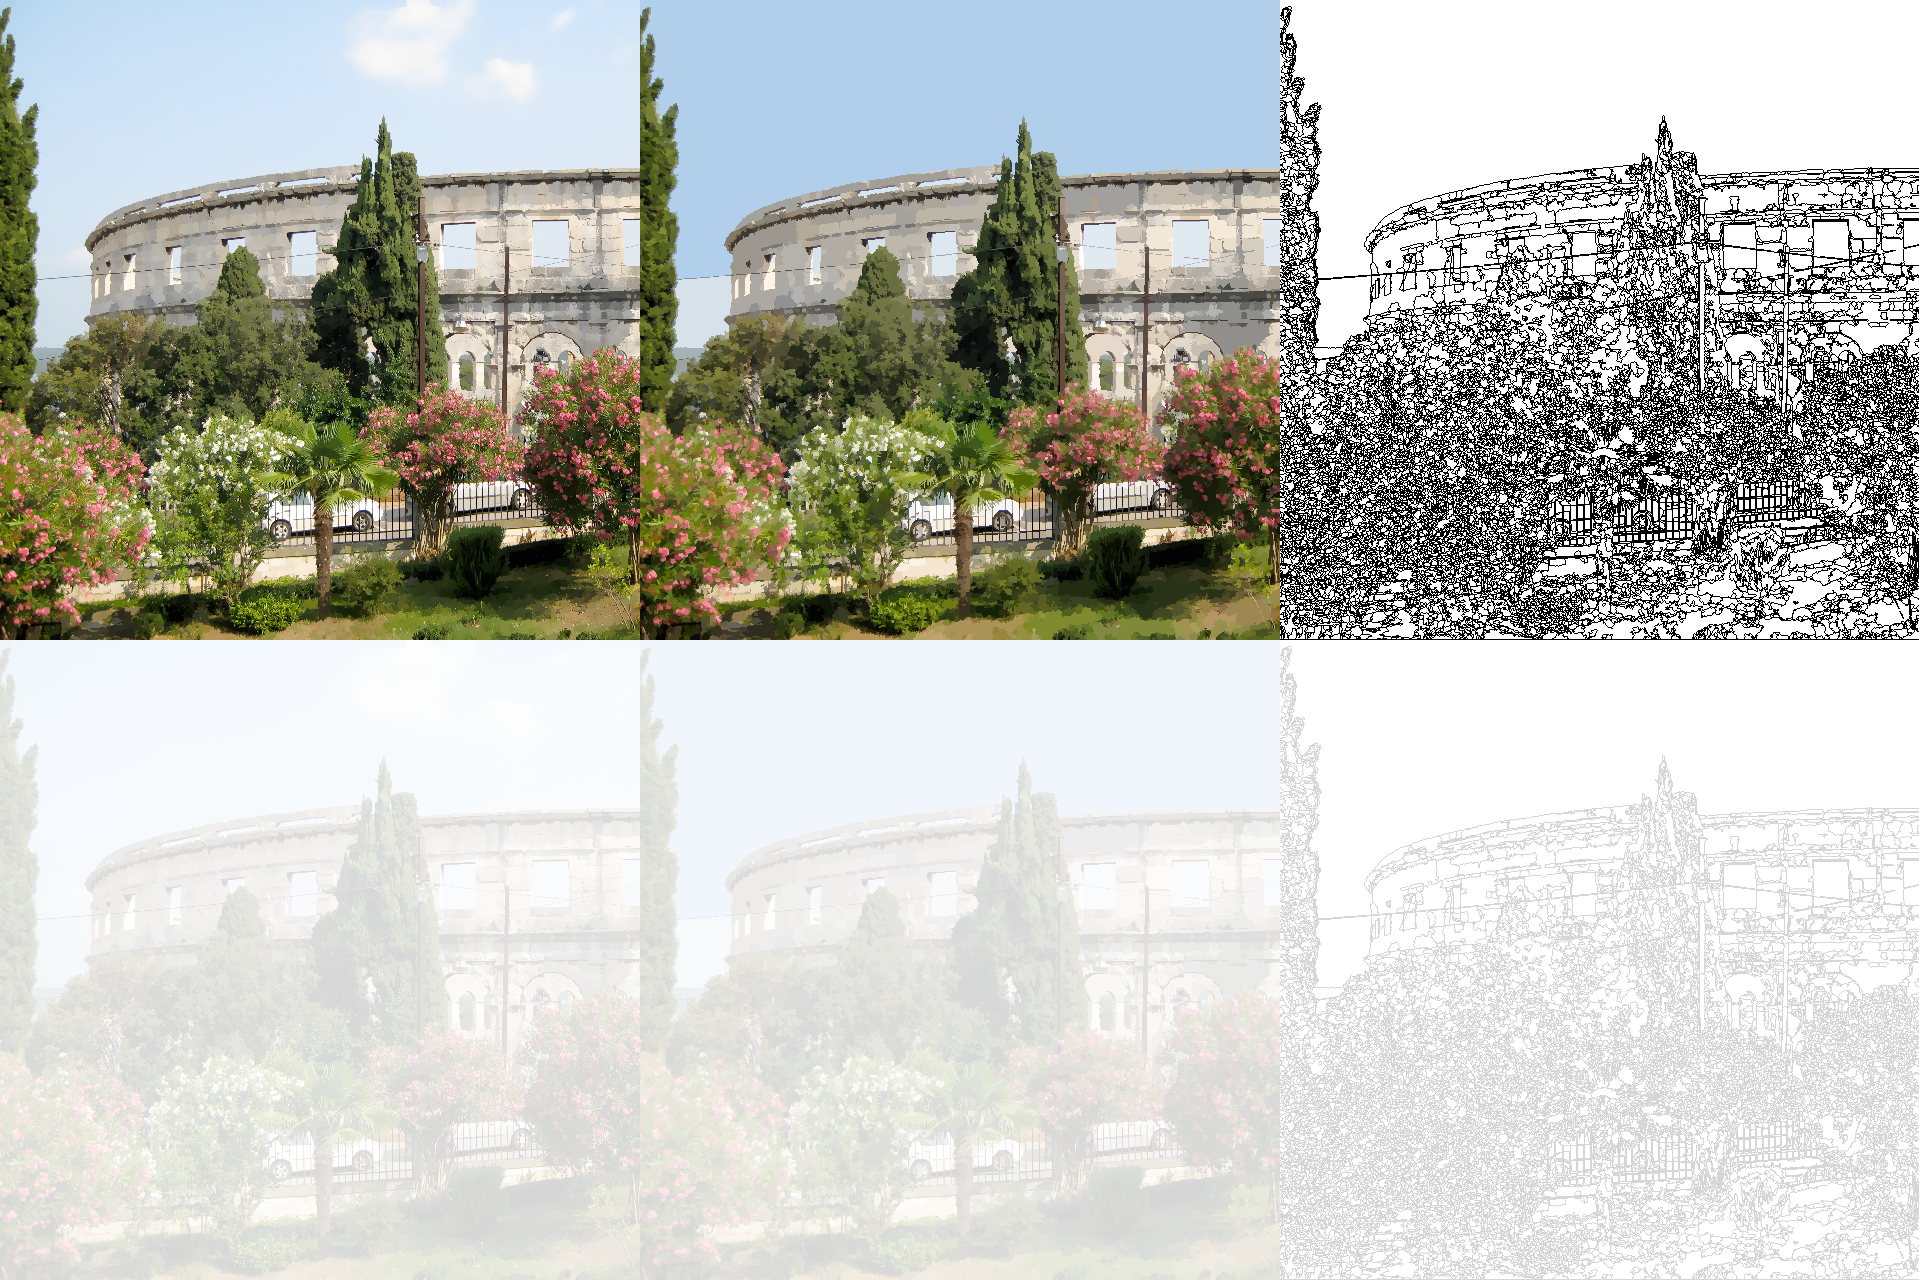
\includegraphics[width=\textwidth]{gfx/appd_fsb_ref.pdf}
  \caption{Result verification. The first row shows the reference pictures
	computed by the \protect\gls{CPU}, (1) the filtered, (2) the segmented image 
	and (3) the edges. Below the annotations made by ImageMagick. In this case
	every pixel computed by the \protect\gls{GPU} matches the reference}
  \label{fig:result_comparison}
\end{figure}

This way it was assured that any modifications or optimizations were done 
correctly and not changing the natural behaviour of the algorithm. 
% subsubsection progress_\&_result_verification (end)
% section the_host (end)

\section{The Device Part} % (fold)
\label{sec:the_device}
For the device part only the filtering step will be further described. As said
before the color conversion is rather simple and can be looked up in any good
computer graphics book. It can be used with minor modifications on the \gls{GPU}. 

The kernel is a single source-code image that runs on each thread on the \gls{GPU}.
The first thing that is done in the kernel is to obtain a unique identifier. 
The identifier is obtained with special functions calls from the hardware. This
unique identifier allows different threads to make different decisions during
kernel execution. The assignment of the unique id to the hardware threads is
deterministic. Thread zero is always the first hardware thread, one can be for
sure that actions which have to be done by a certain thread are really done
by the corresponding thread in the hardware. 

The unique id is as well important for data distribution. 
In \autoref{sec:cuda_thread_hierarchy} it was shown that one thread is responsible
for a single pixel. So there are so many threads as there are pixel in the image 
where the threads are numbered from 0--(number of pixel - 1). Every thread having
its unique id which is at the same time the position in the array of pixel can
now easily fetch the pixel from global memory for computation. 

Each thread takes the \gls{LUV} values and calculates the mean shift vector 
until convergence. When a thread finishes execution it saves the convergence 
point to a second buffer to the same place in the array (unique id) where the 
thread fetched the input pixel. 

For the first shot no other memories where used to improve performance. The first
implementation was just to make it work. The next chapter will digg deeper into
the hardware and optimize the code to run efficiently. The performance
and scalability is evaluated in a subsequente chapter. 
% section the_device (end)
% chapter implementation (end)

\section{Summary} % (fold)
\label{sec:summary}
After an extensive analysis and a good design the effort to implement the algorihtm
was not so big. The most difficult part was the implementation of the
mean shift method in the reference implementation. It had to be verified that
the algorithm is working and doing the right stuff. 

After that it was crucial to get in touch with \gls{CUDA} and all dependent
libraries and to know what function is exactly doing and how to use it. 

Merging the reference implementation with \gls{CUDA} was pretty easy as \gls{CUDA}
is just a extension to C and only some keywords where introduced that have to 
be used in the right way. 

The programming flow of first moving data to the \gls{GPU}, processing and then
getting the data back to the host was already known, from implementing a raytracer
on the Cell processor. Pretty all accelerators have a similar programming flow. 

Luckily there was the reference implementation which was used for result verification
not only for the filtering part but as well for the other two kernels where a bug
was easily spotted in form of red pixels thanks to the great tools of ImageMagick.


% section summary (end)















